\chapter{Experiments and Results}
\label{chap:experiments}
In this chapter, the experiment setup and results are described in detail. In section \ref{sec:setup}, the datasets, developing environment, metrics, and implementation details are explained. Section \ref{sec:training_original_egovit} presents the results of the original EgoViT on the EGTEA Gaze+ dataset. In Section \ref{sec:training_egovit_with_gaze}, the results of the enhanced EgoViT training with gaze information are presented. Finally, the results of the experiments are analyzed and discussed in Section \ref{sec:Disscussion}.

% In this chapter, we describe the experimental setup and the results of our experiments. We start by describing the experimental setup in Section~\ref{sec:setup}. Then, we present the results of training the original EgoViT model on the EGTEA Gaze+ dataset in Section~\ref{sec:training_original_egovit}. In Section~\ref{sec:training_egovit_with_gaze}, we present the results of training the EgoViT model with gaze information.

\section{Setup}
\label{sec:setup}
\textbf{Datasets} The largest commonly used egocentric video dataset is EPIC-KITCHENS \cite{Damen2018EPICKITCHENS}, which contains videos of daily activities from multiple participants in their natural environment. However, this dataset does not provide gaze data from the videos. For this reason, the EGTEA Gaze+ \cite{li_eye_2020} dataset is utilized in this thesis. EGTEA Gaze+ is a large and comprehensive dataset for \gls{fpv} actions and gaze tracking. It includes HD videos, gaze tracking data, and frame-level action annotations. The dataset consists of 86 unique sessions from 32 subjects across 7 recipes. The annotations include 10321 action instances from 106 action categories, with an average action instance duration of 4.2 seconds. There are three non-overlapping train and test sets available, with 8299/2022, 8299/2022 and 9230/2021 samples (train/test). These splits are generated through random sampling, ensuring that approximately  80\% of the samples per category are included. The split set 1 is used in this thesis for training and testing. For all Experiments, this study follows prior work by reporting top-1 accuracy, top-5 accuracy and average mean class accuracy.

\textbf{Developing Environment} The experiments are conducted on a GPU server in SimTech Stuttgart. The server runs Ubuntu operating system, and the model with its experiments are implemented in Python 3.9. The deep learning framework PyTorch 2.2 and CUDA 12.1 are used for the implementation.
The important ependencies and their versions are listed below:
\begin{itemize}
    \item torch==1.10.0
    \item torchvision==0.17.0
    \item numpy==1.26.4
    \item pandas==2.2.1
    \item opencv-python==4.10.0.82 
\end{itemize}

\textbf{Implementation Details} The video clips in  EGTEA Gaze+ dataset have an average length of 3.2 seconds, although some clips are significantly longer. To handle this, the video clips are uniformly sampling into 32 frames. The frames are resized to $224 \times 224$ pixels, resulting in an input tensor of shape $32 \times 3 \times 224 \times 224$. Dimension 3 represents the RGB channels of the image. Another input tensor contains gaze tracing data with a shape of $32 \times 1 \times 1$, where $1 \times 1$ represents gaze coordinates $(x,y)$in each frame. The gaze coordinates are normalized to the range of $[0, 1]$. 

Frame extraction from the video clips and the processing of gaze features can be time-consuming during training. To reduce the training time, frame extraction and gaze-hand-object features processing are performed offline and saved as a NumPy zipped (.npz) file. And the action label is also read and saved in this zipped file. Thus, the image, gaze-hand-object features, and action label of one video clip are saved in a single file. The structure of the NumPy zipped (.npz) file is as follows:
\begin{align*}
    \text{Preprocessed Data:} & (\text{frames}: [32, 3, 224, 224], \quad \text{features}: [32, 3, 2048], \quad \text{label}: [1])
\end{align*}
The training process opens the data file only once for each video clip, significantly reducing the training time. All experiments are conducted on the prepared data.

The models are trained using the AdamW \cite{loshchilov_decoupled_2019} optimizer.  The learning rate is set to $1 \mathrm{e}{-5}$, and the batch size is set to 4. The layers the in Video Swin Transformer use the pretrained weights from KINETICS400\_V1. The models are trained for 20 epochs. In some experiments, a cosine decay learning rate scheduler with a linear warm-up of 2.5 epochs is used, following the approach in \cite{liu_video_2021}. The stochastic depth rate and weight decay are adopted as in \cite{liu_video_2021}, set to 0.3 and 0.05 respectively. The configuration of Swin-B is used. The architecture hyperparameters of Swin-B are as follows:
\begin{align}
    \text{Swin-B:} &\quad C = 128, \quad \text{layer numbers} = \{2, 2, 18, 2\}
\end{align}
Where $C$ represents the $C$-dimentional features (see Figure \ref{fig:swin-transformer}), and $\{2, 2, 18, 2\}$ represents the number of times the Transformer Block is repeated in each stage.

\textbf{Metrics} For inference, the same data structure as used in training is applied. The model is evaluated on the test split1 of the EGTEA Gaze+ dataset. The top-1 accuracy, top-5 accuracy, and mean class accuracy are calculated. The top-1 accuracy is the proportion of correctly predicted class (with the highest predicted probability) among all samples. It is the most straightforward accuracy metric. The calculation of top-1 accuracy is:
\begin{align}
    \text{Top-1 Accuracy} = \frac{\text{Number of correctly predicted samples}}{\text{Total number of samples}}
\end{align}
Top-5 accuracy refers the percentage of instances where the true class label is within the top five predicted class label. The formula for top-5 accuracy is:
\begin{align}
    \text{Top-5 Accuracy} = \frac{\text{Number of correctly predicted samples in top-5}}{\text{Total number of samples}}
\end{align}
The mean class accuracy is the average accuracy for each class. It accounts class imbalance by assigning equal weight to each class. The formula for mean class accuracy is:
\begin{align}
    \text{Mean Class Accuracy} = \frac{1}{N} \sum_{i=1}^{N} \frac{\text{Number of correctly predicted samples for class i}}{\text{Total number of samples in class i}}
\end{align}
Where $N$ is the number of classes. 
\clearpage
In this thesis, a series number of experiments are conducted. Different models are trained with different features and configurations. For a simple discription of the experiments, the experiments ID are denoted and explained in the Table \ref{tab: exp_id}. The experiments ID are used to identify the experiments in the following sections. When not mentioned, the experiments are trained with gaze version 1, with pretrained weights from KINETICS400\_V1, and a fixed learning rate of $1 \mathrm{e}{-5}$.
\vspace{5mm}
\begin{table}[htbp]
    \centering
    \caption{Experiments ID and Description}
    \begin{tabular}{ll}
    \hline\hline
    Experiment ID & Description \\
    \hline
    Orig\_HO\_no\_pretrain  & Original EgoViT: without pretrained weights \\
    Orig\_HO                & Original EgoViT: pretrained weights \\
    Orig\_HO\_sched. LR     & Original EgoViT: pretrained weights and scheduler LR \\
    Enh\_GHO             & Enhanced EgoViT: GHO features \\
    Enh\_G               & Enhanced EgoViT: G features \\
    Enh\_GHO\_v2         & Enhanced EgoViT: GHO features and gaze\_v2 \\
    Enh\_G\_v2           & Enhanced EgoViT: G features and gaze\_v2 \\
    Enh\_v2\_GHO\_v2     & Enhanced EgoViT\_v2: GHO features and gaze\_v2 \\
    Enh\_v3\_HO          & Enhanced EgoViT\_v3: HO features \\
    Enh\_v3\_GHO\_v2     & Enhanced EgoViT\_v3: GHO features and gaze\_v2 \\
    Enh\_v3\_G\_v2       & Enhanced EgoViT\_v3: G features and gaze\_v2 \\
    \hline\hline
    \end{tabular}
    \label{tab: exp_id}
\end{table}
\clearpage


\section{Training the Original EgoViT with EGTEA Gaze+ Dataset}
\label{sec:training_original_egovit}
Because the code for the original EgoViT is not publicly available, an approximate model is first built in this thesis. To compare the effect of gaze information, the original EgoViT from \cite{pan_egovit_2023} is trained on the EGTEA Gaze+ dataset and used as the baseline for all experiments. Therefore, only frames and hand-object features in the video clips are fed into the original EgoViT model.

The original EgoViT model is first trained without pretrained weights from KINETICS400\_V1, using a learning rate of $1 \mathrm{e}{-5}$ for all layers. The model is trained for 40 epochs. Figure \ref{fig:orig-EgoViT} shows the training loss and accuracy of the original EgoViT model. The rot line represents the training loss, and the blue line represents the training accuracy. The model converges rapidly in the first 5 epochs and the loss decreases consistently between 5 and 30 epochs. After 30 epochs, the model converges slowly to the minimum loss. The accuracy follows a similar trend, inversely related to the loss.

\begin{figure}[b]
    \centering
    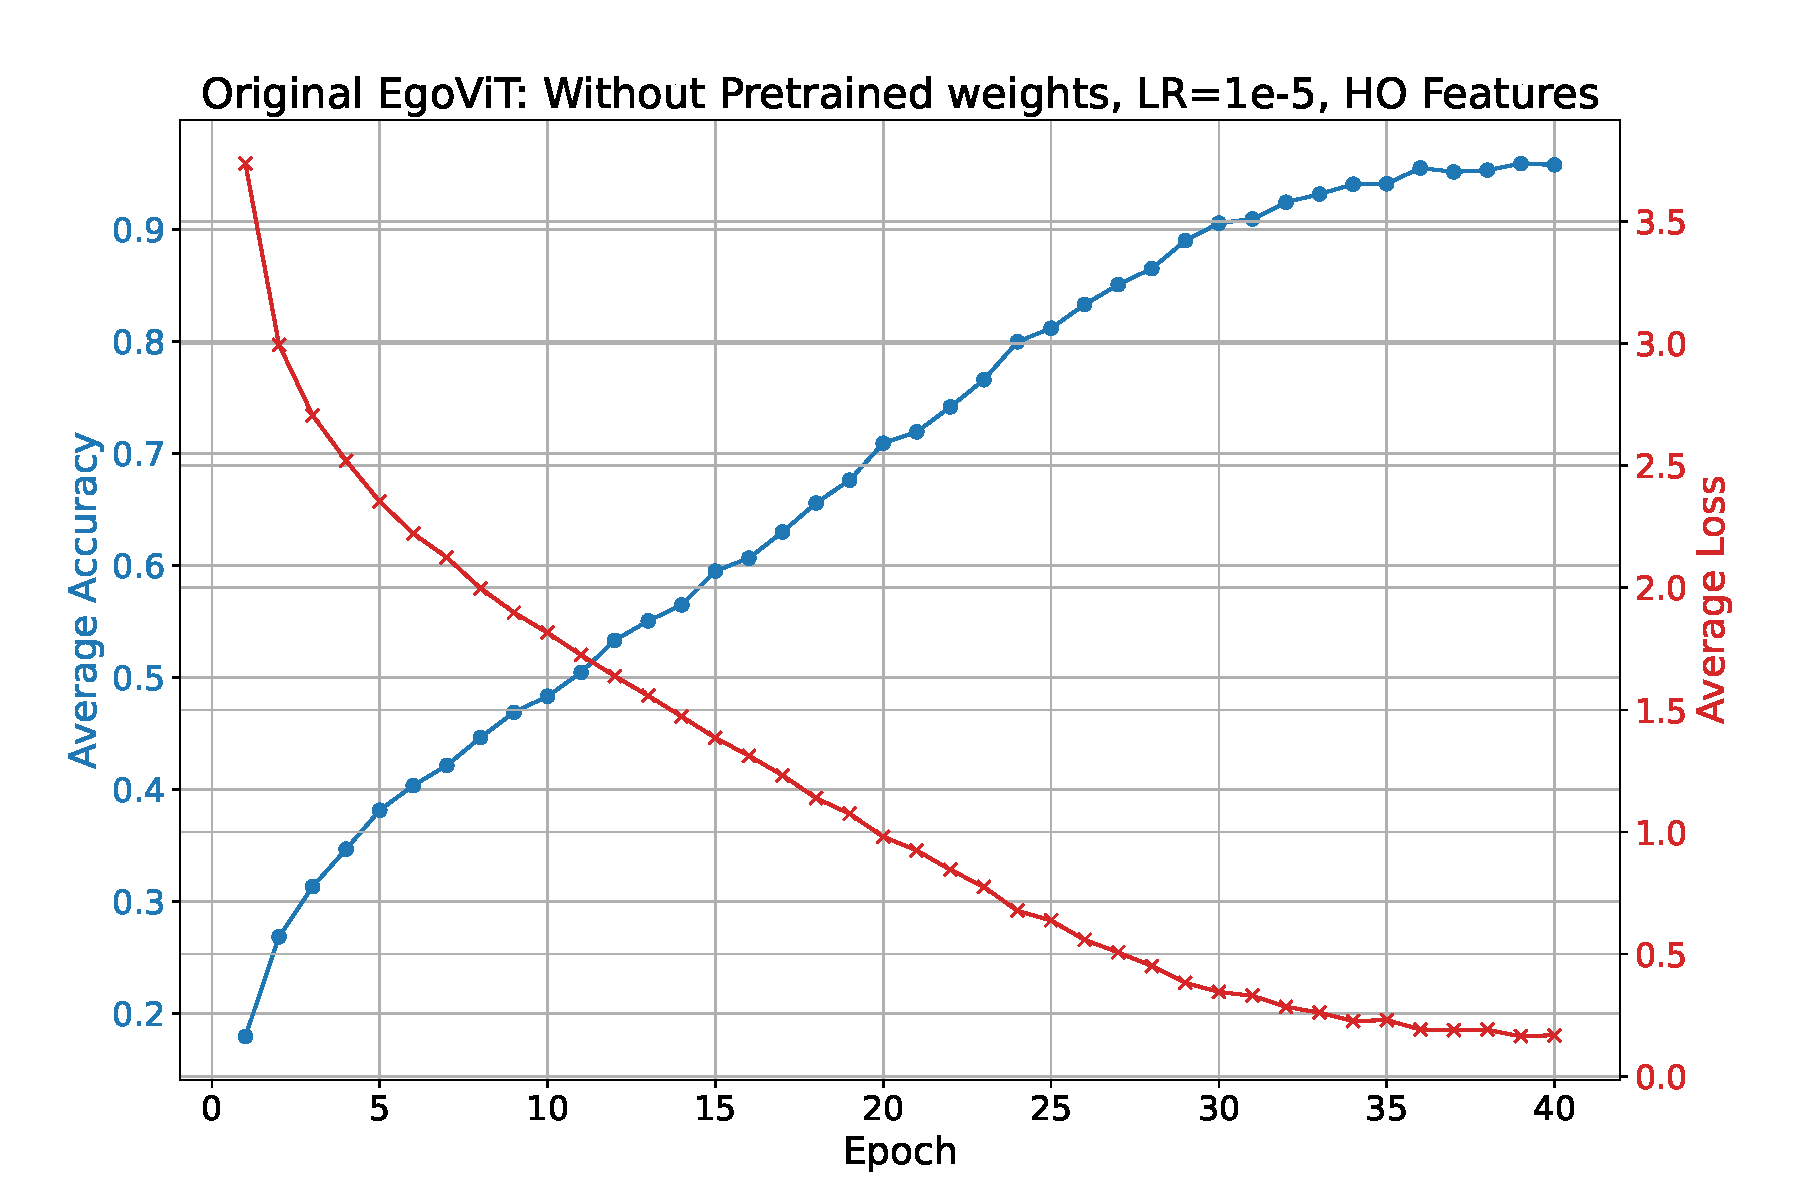
\includegraphics[width=0.9\textwidth]{graphics/figure11}
    \caption{The training loss and accuracy curves for the original EgoViT model trained without pretrained weights. The model is trained over 40 epochs with a learning rate of 1e-5. Blue curve: training accuracy, red curve: training loss.}
    \label{fig:orig-EgoViT}
\end{figure}
\clearpage
\begin{figure}[htbp]  
    \centering
    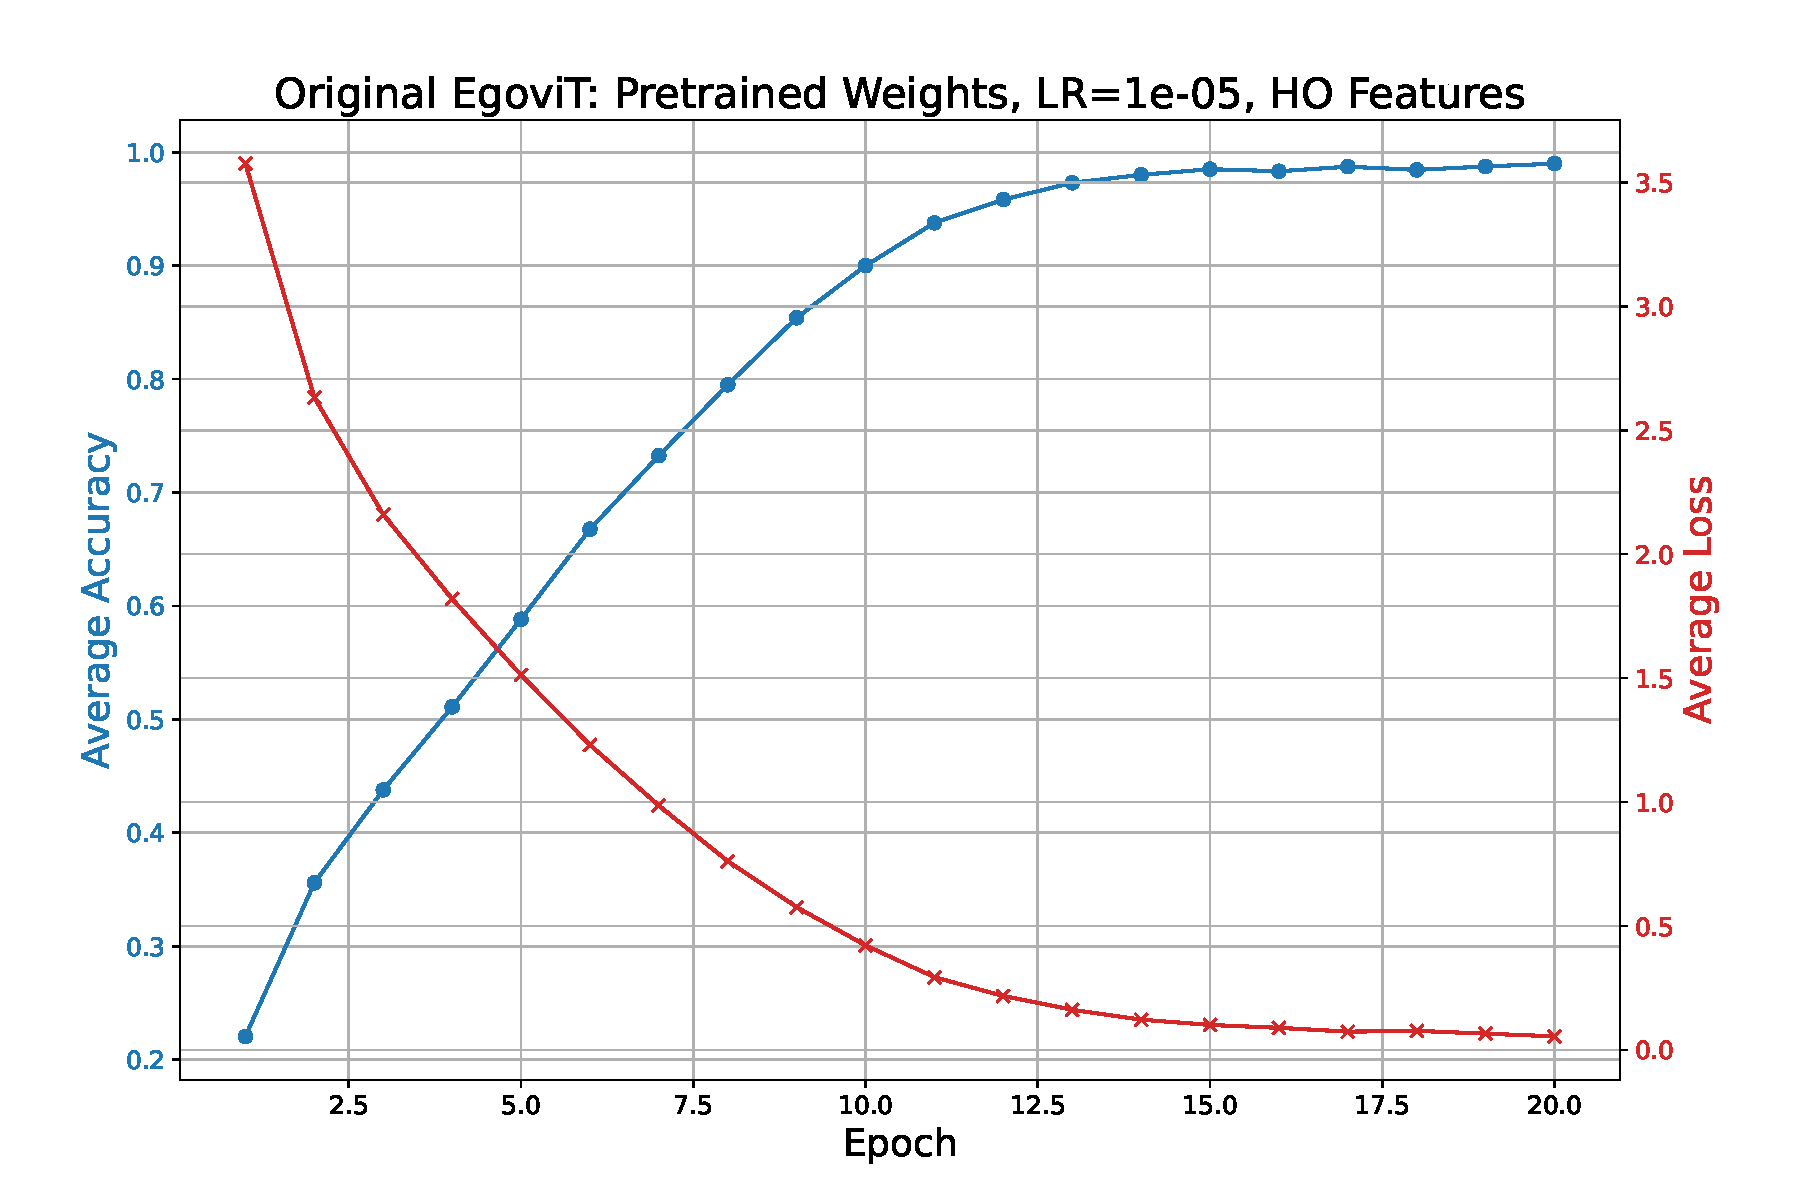
\includegraphics[width=0.9\textwidth]{graphics/figure31}
    \caption{The training loss and accuracy curves for the original EgoViT model trained with pretrained weights. The model is trained over 20 epochs with a learning rate of 1e-5. Blue curve: training accuracy, red curve: training loss.}
    \label{fig:orig-EgoViT-with-pretrained}
\end{figure}
\vspace{3mm}
To improve the training performance, the original EgoViT model is trained with pretrained weights from KINETICS400\_V1, while maintaining a learning rate of $1 \mathrm{e}{-5}$. The model is trained for 20 epochs. Figure \ref{fig:orig-EgoViT-with-pretrained} shows the training loss and accuracy of the original EgoViT model with pretrained weights. The loss decreases rapidly in the first 3 epochs and then follows a shorter, consistently decreasing period. After 20 epochs, the model converges slowly to the minimum loss. The accuracy follows a similar trend, inversely related to the loss. By the 13th epoch, the model is almost fully converged and then decreases slowly to the minimum. This result indicates that the model with pretrained weights performs better than the model without them. Therefore, in the following experiments, the model with pretrained weights is used.

\clearpage
\begin{figure}[htbp]
    \centering
    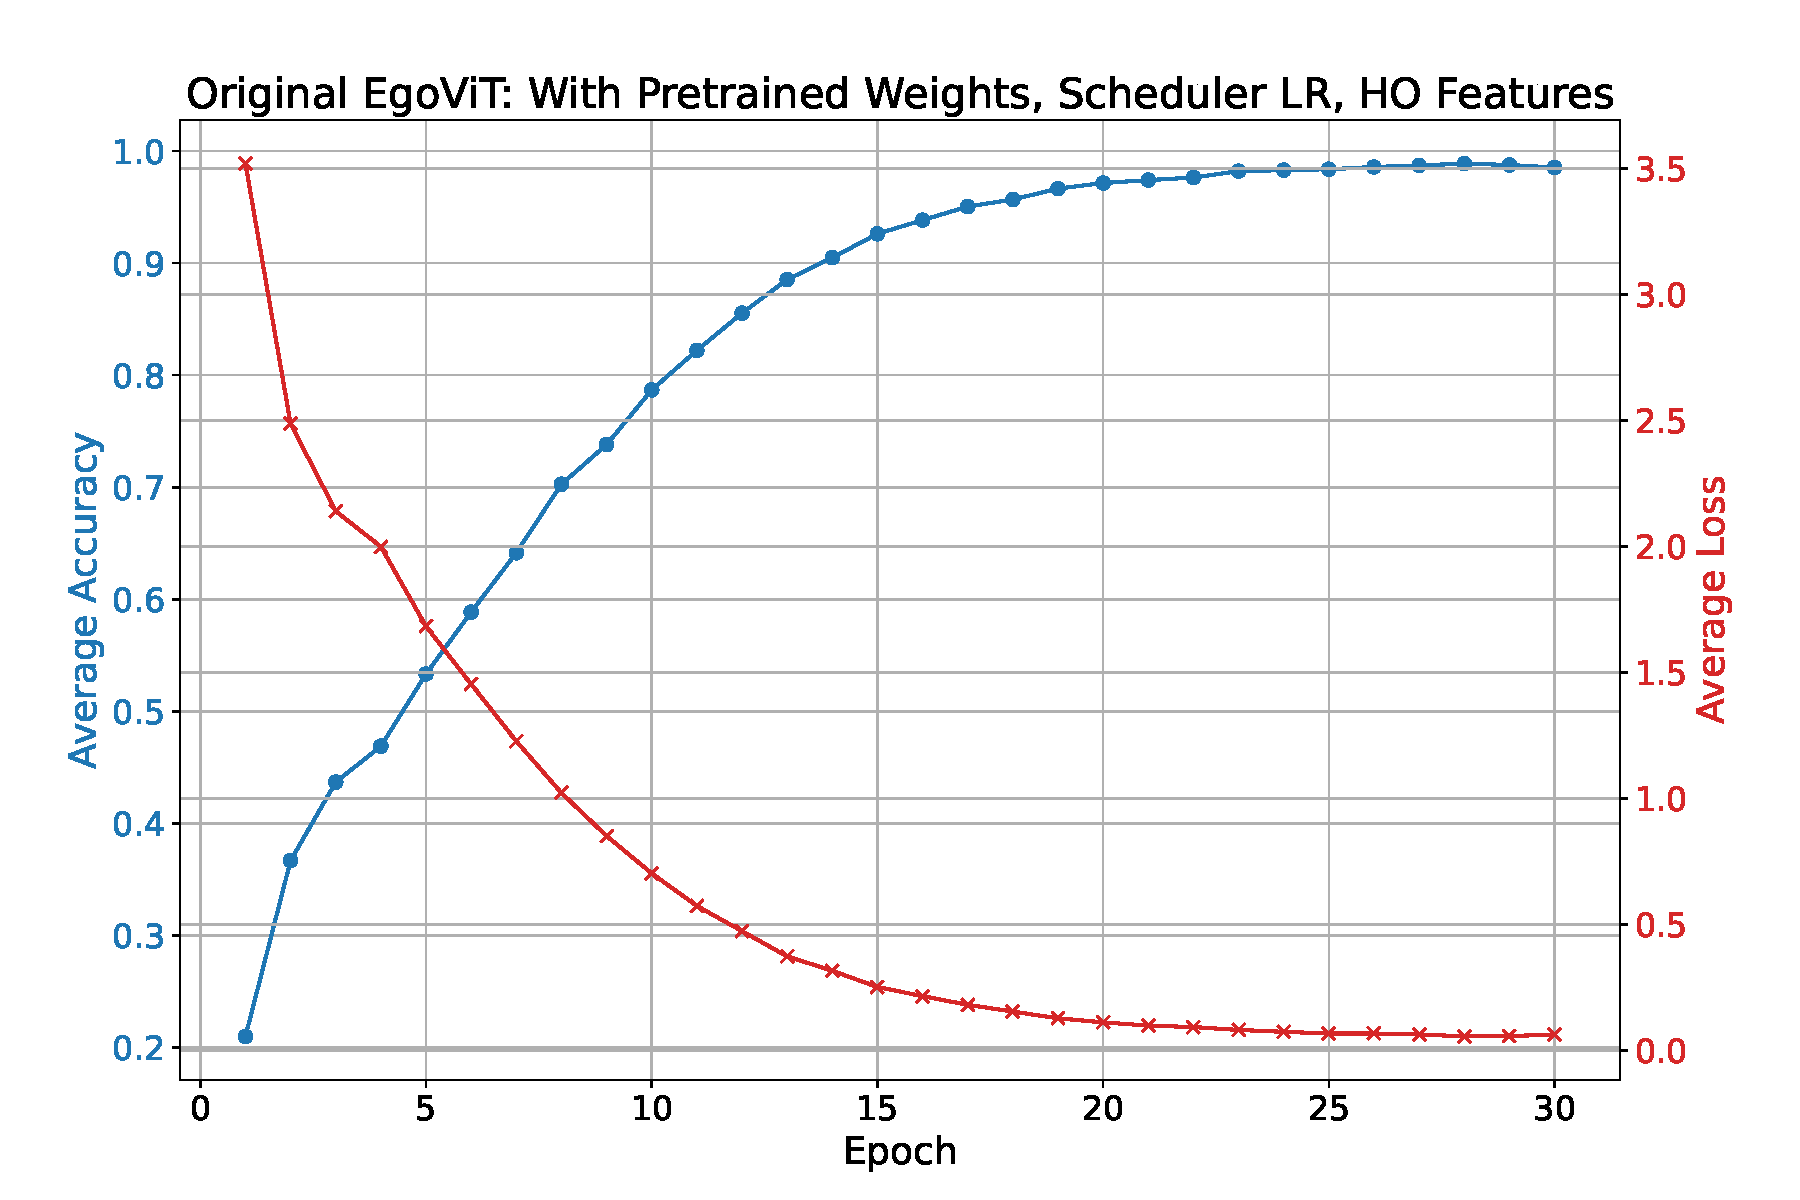
\includegraphics[width=0.9\textwidth]{graphics/figure21}
    \caption{The training loss and accuracy curves for the original EgoViT model trained with pretrained weights. The model is trained over 30 epochs with a scheduler learning rate. Blue curve: training accuracy, red curve: training loss.}
    \label{fig:orig-EgoViT-no-pretrained}
\end{figure}
\vspace{3mm}
The learning rate is another hyperparameter that affects model performance. A cosine scheduler learning rate, as described in \cite{liu_video_2021}, is applied to fine-tune the learning rate. The model is trained for 30 epochs. Figure \ref{fig:orig-EgoViT-no-pretrained} shows the training loss and accuracy of the original EgoViT model with pretrained weights and scheduler learning rate. In the first 10 epochs, the loss decreases rapidly. After 15 epochs, the model converges slowly to the minimum loss. Between 20 and 25 epochs, the model achieves maximum accuracy and minimum loss.

\clearpage
The testing results of three training methods are shown in Table \ref{tab:original-egovit}. The model with pretrained weights and a scheduler learning rate achieves the highest top-1 accuracy of 0.517, followed by the model with pretrained weights and a fixed learning rate of 0.515. The model with pretrained weights and a scheduler learning rate has the worst performance, achieving the lowest top-1 accuracy, top-5 accuracy, and mean class accuracy of 0.484, 0.744, and 0.358, respectively. All three metrics follow a similar trend, with the model using a fixed learning rate of $1 \mathrm{e}{-5}$ showing better performance overall. While the pretrained weights from KINETICS400\_V1 did not improve \gls{ear} in inference, they accelerated the training process. One possible reason for the lower performance of the scheduler learning rate is that the Video Swin Transformer is divided into two parts and the model has many additional, making the scheduler learning rate configuration from \cite{liu_video_2021} potentially unsuitable for the original EgoViT model. A new configuration for the scheduler learning rate could be explored in future work.
\newline

\begin{table}[h]
    \centering
    \caption{Test Results of original EgoViT with HO Features}
    \begin{tabular}{lccc}
    \hline\hline
    Experiment ID & Top-1 Acc.(\%) & Top-5 Acc.(\%) & Mean Class Acc.(\%) \\
    \hline
    Orig\_HO\_no\_pretrain       & 51.5 & 78.5 & 38.8 \\
    Orig\_HO                     & 51.7 & 75.2 & 40.6 \\
    Orig\_HO\_sched. LR          & 48.4 & 74.4 & 35.8 \\
    \hline\hline
    \end{tabular}
    \label{tab:original-egovit}
\end{table}

\section{Training the Enhanced EgoViT with Gaze Information}
\label{sec:training_egovit_with_gaze}
In this section, the enhanced EgoViT is trained with additional gaze information using different methods to evaluate the effect of gaze information on the model. In this series of experiments, two types of gaze data are used for training and testing. The first type, referred to as gaze version 1, contains only the gaze tracking type of fixation. Thus, some sampled frmes may not have gaze data. The second type, referred to as gaze version 2, includes both fixation and saccade types of gaze tracking. Gaze version 2 has more collected gaze data from the dataset but also includes some frames that lack gaze data. For these frames, the missing gaze data is ignorded and gaze features are randomly generated, resulting in a highter overall quality of gaze data compared to gaze version 1.

For an ablation study, the enhanced EgoViT is trained with gaze-hand-object features and only gaze features seperetly. The model is trained for 20 epochs with a learing rate of $1 \mathrm{e}{-5}$. The training loss and accuracy of the enhanced EgoViT model with gaze-hand-object features and gaze features are shown in Figure \ref{fig:egovit-with-gho} and \ref{fig:egovit-with-gaze}. The both training have a similar loss and accuracy curved line compared with the experiment orig\_pretrain\_HO in Figure \ref{fig:orig-EgoViT-with-pretrained}. The three experiments have similarity loss converge rate and all reach the minimum loss after 15 epochs. The top-1, top-5 and mean class accuracy of the two experiments are shown in Table \ref{tab:Results_table2}. The model with hand-object features achieves the highest top-1 accuracy of 0.517 and the highest mean class accuracy of 0.406, followed by the model with gaze-hand-object features, which achieves 0.514 and 0.400, respectively. However, the gaze-hand-object model has the highest top-5 accuracy of 0.767. The model with only gaze features has the lowest scores across all three metrics, with a top-1 accuracy of 0.489, a top-5 accuracy of 0.751, and a mean class accuracy of 0.377. \newline
\begin{table}[h]
    \centering
    \caption{Test Results on Models with Different Features}
    \begin{tabular}{lccc}
    \hline\hline
    Experiment ID & Top-1 Acc. & Top-5 Acc. & Mean Class Acc. \\
    \hline
    Orig\_HO        & 51.7 & 75.2 & 40.6 \\
    Enh\_GHO     & 51.4 & 76.7 & 40.0 \\
    Enh\_G       & 48.9 & 75.1 & 37.7 \\
    \hline\hline
    \end{tabular}
    \label{tab:Results_table2}
\end{table}

% \clearpage
\begin{figure}
    \centering
    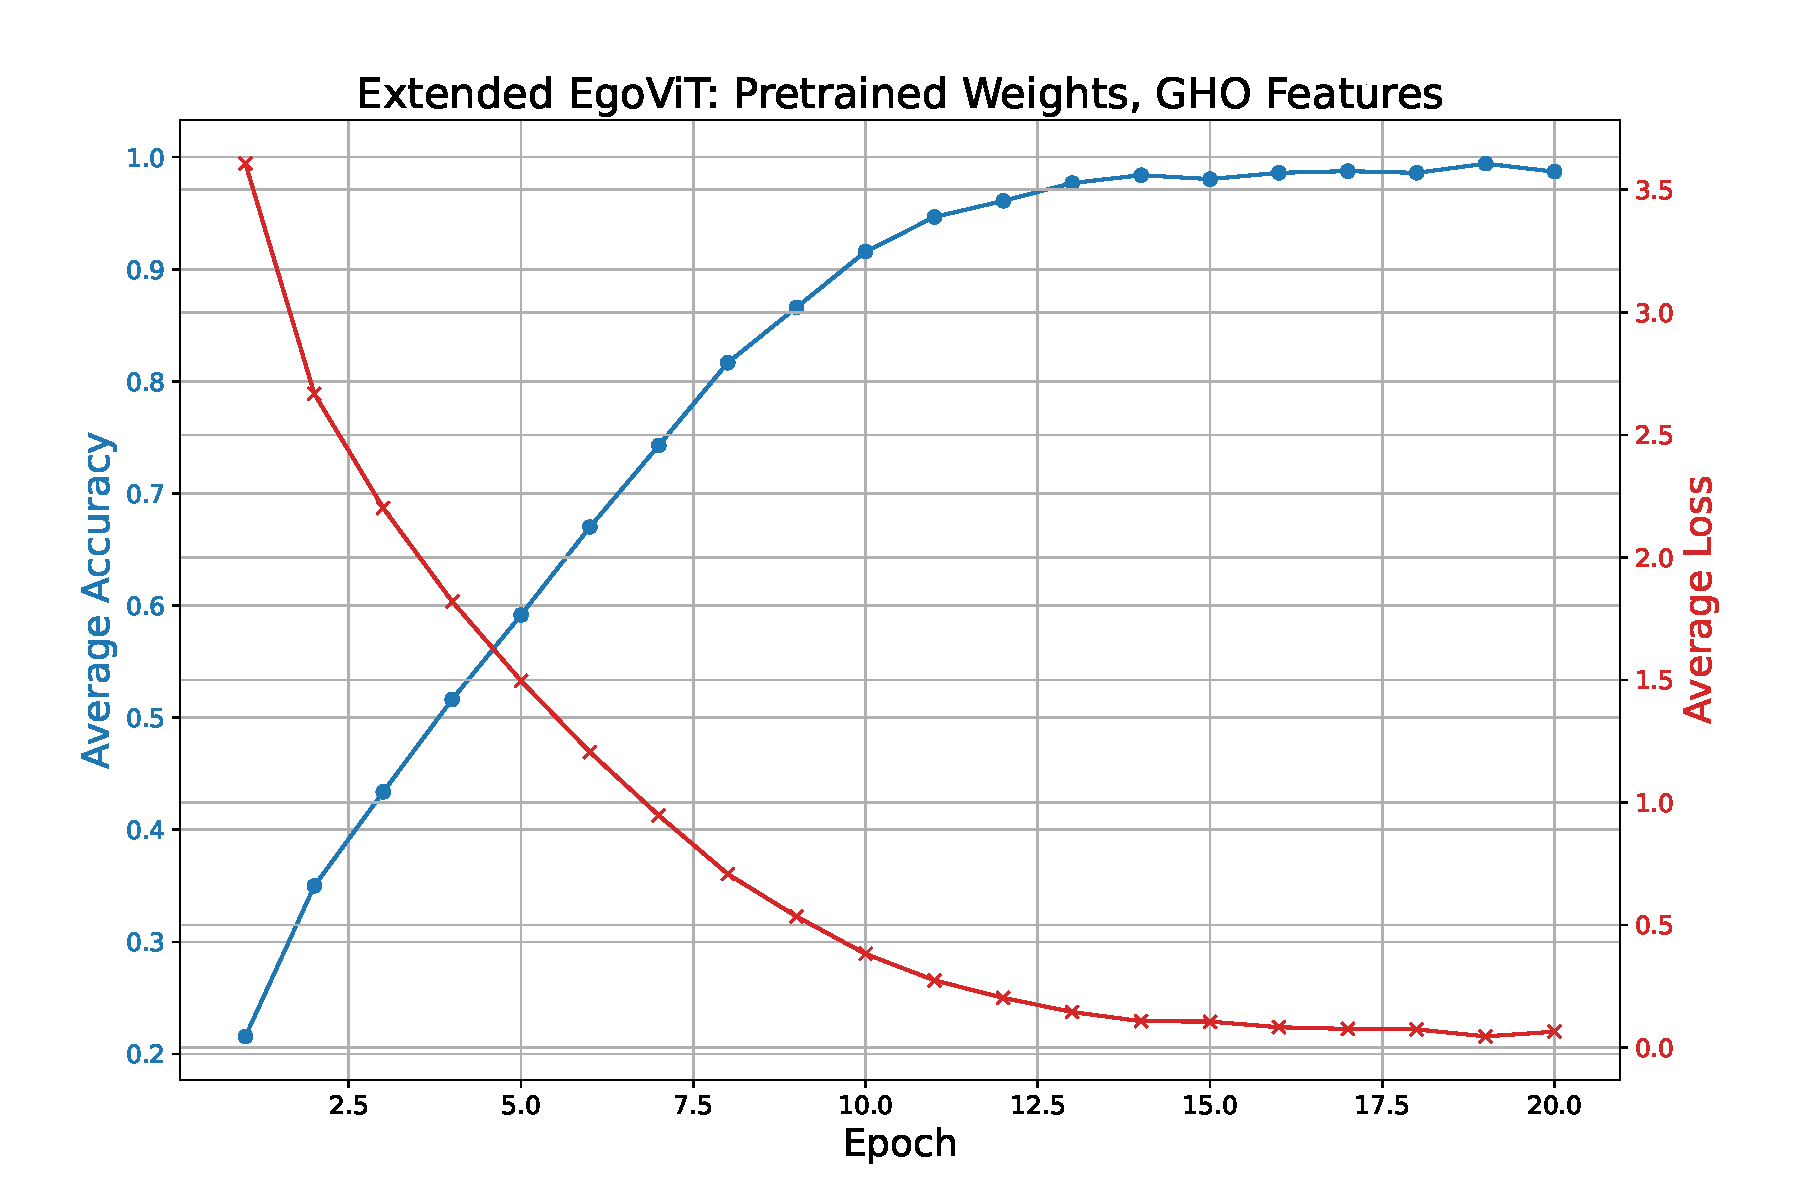
\includegraphics[width=0.9\textwidth]{graphics/figure41}
    \caption{Training loss and accuracy of the enhanced EgoViT with gaze-hand-object features. Blue curve: training accuracy, red curve: training loss.}
    \label{fig:egovit-with-gho}
\end{figure}
\begin{figure}
    \centering
    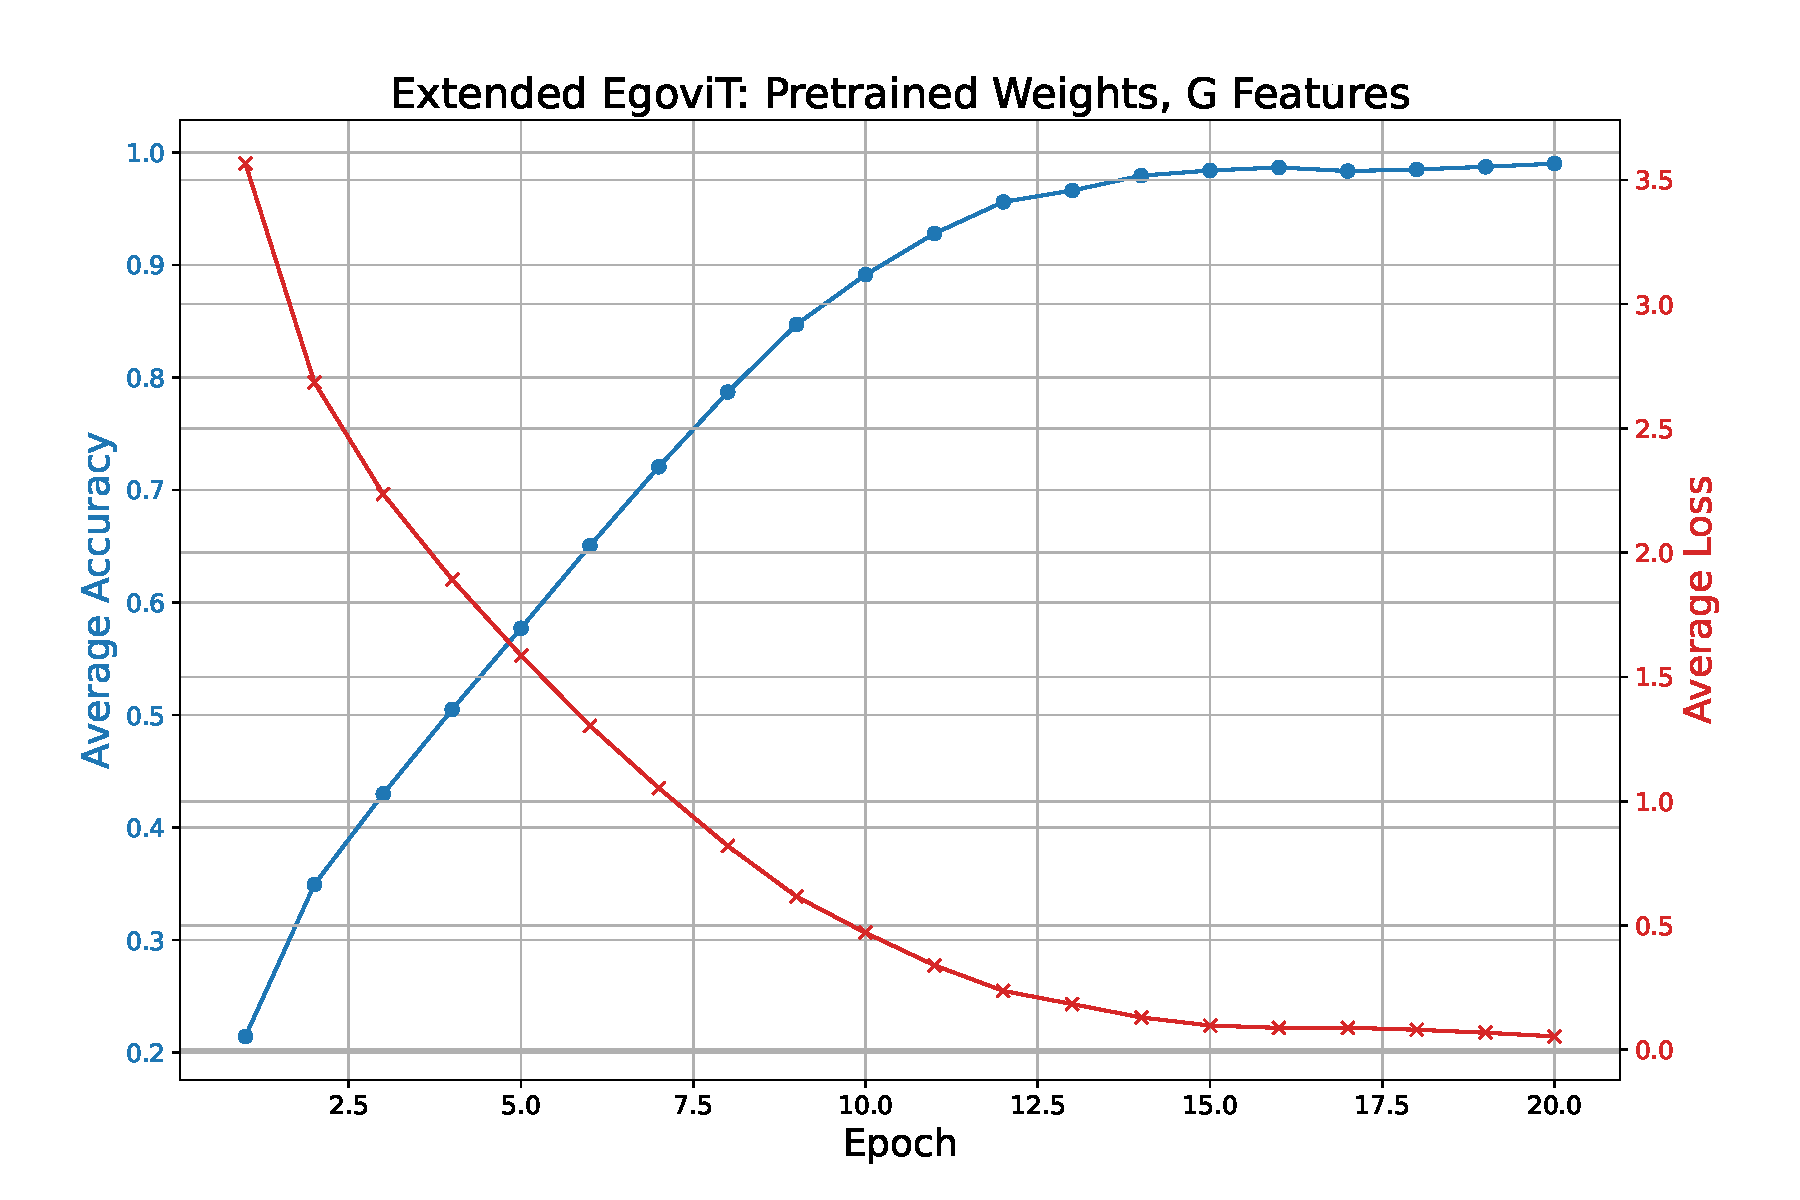
\includegraphics[width=0.9\textwidth]{graphics/figure51}
    \caption{Training loss and accuracy of the enhanced EgoViT with gaze features. Blue curve: training accuracy, red curve: training loss.}
    \label{fig:egovit-with-gaze}
\end{figure}
\newpage
\begin{figure}[htbp]
    \centering
    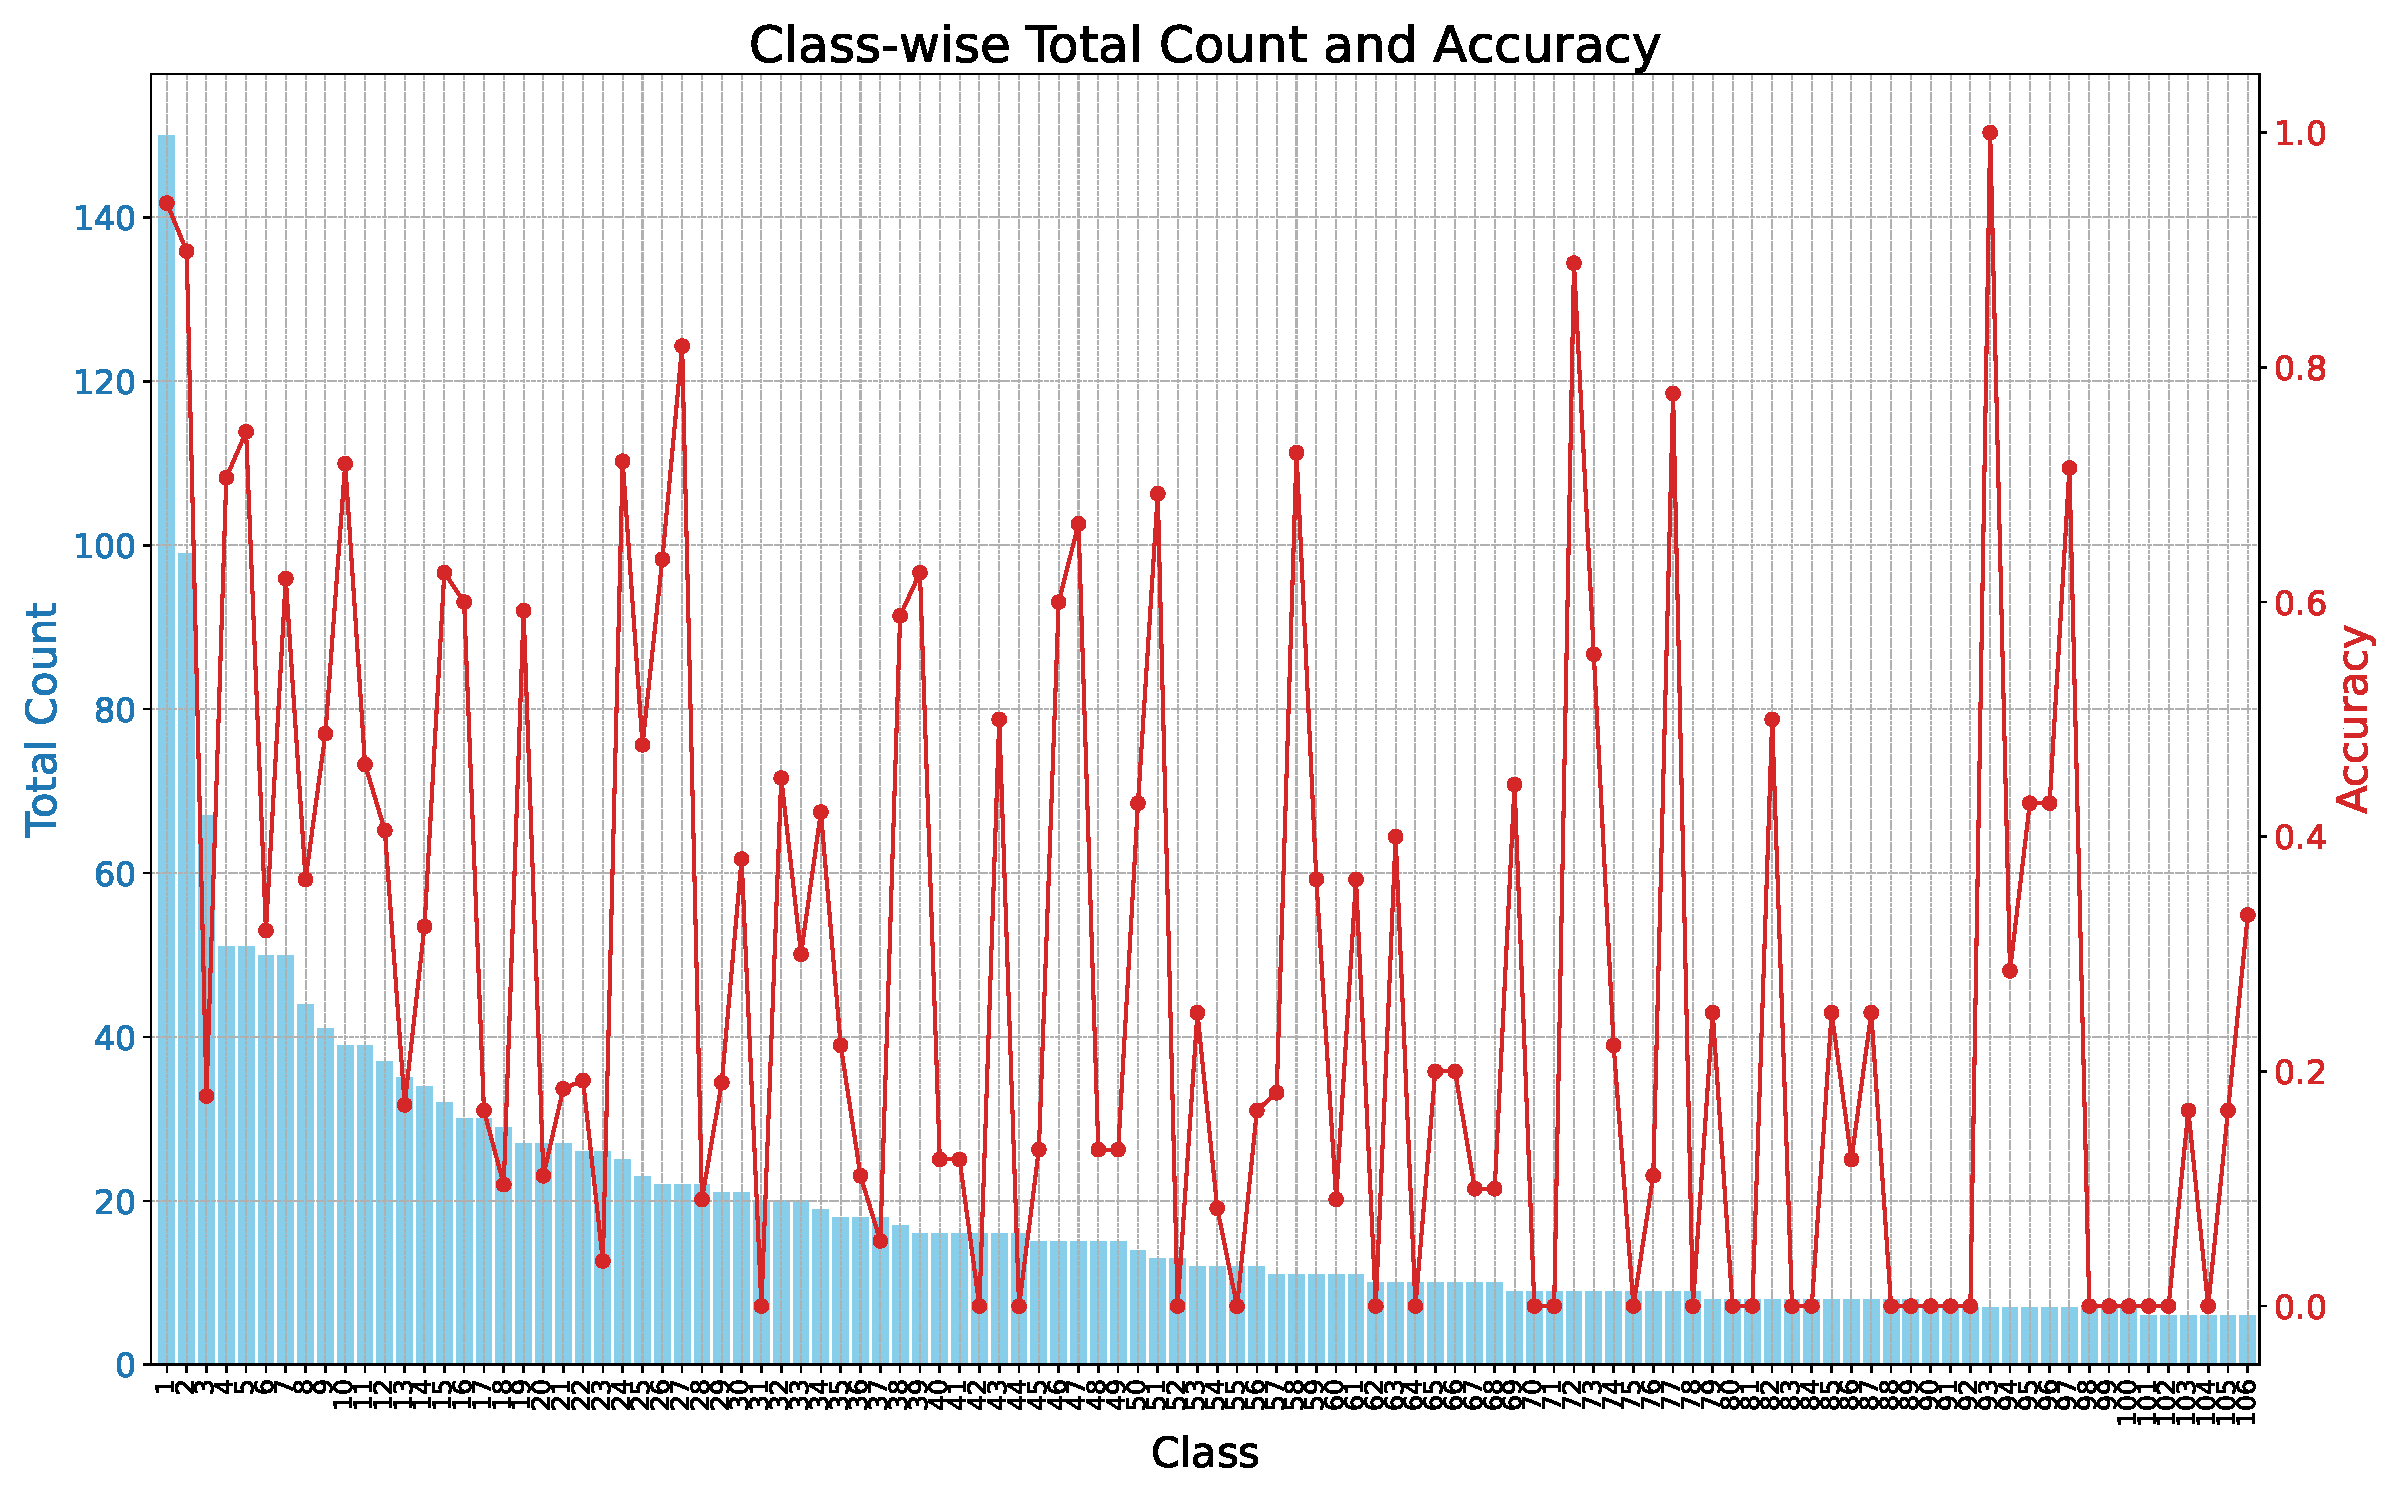
\includegraphics[width=\textwidth]{graphics/2in1}
    \caption{The class-wise total count (blue bars) and accuracy (red line) of the enhanced EgoViT model. The x-axis represents the different classes, while the left y-axis shows the total count of instances per class, and the right y-axis shows the accuracy for each class. }
    \label{fig:action_class}
\end{figure}
\vspace{3mm}
The number of samples for each action class (a total of 106 classes) in the test split1 is calculated and shown in Figure \ref{fig:action_class}. The x-axis represents the action class, and the y-axis represents the number of samples in each class. The top-1 accuracy of the model with gaze-hand-object features is indicated by the red line in Figure \ref{fig:action_class}. This figure shows the number of samples for each action class and the corresponding accuracy of the model with gaze-hand-object features. Class label 1 has the highest number of samples at 150, while the other classes have significantly fewer samples. From class label 31 to 106, the number of samples is under 20. The accuracy of action recognition for many classes with fewer samples is low, with some classes having an accuracy of 0. Since the distribution of samples in each class in train split1 is similar to that in test split1, the model is not able to effectively learn the features of classes with fewer samples.

Two experiments are conducted to explore the effect of gaze quality on the model. The enhanced EgoViT is trained with gaze-hand-object features and only gaze features, using gaze data extracted from gaze version 2. The hyperparameters for training remain the same as in the previous experiments. Table \ref{tab:Results_table3} shows the results and compares them with the results of the experiments Enh\_GHO and Enh\_G. The top-1 accuracy indicates that the model trained with gaze version 2 performs better than the model trained with gaze version 1.
The experiment Enh\_GHO\_v2 achieves a top-1 accuracy of 0.520, which is 0.6\% higher than the experiment Enh\_GHO. The experiment Enh\_G\_v2 achieves a top-1 accuracy of 0.500, which is 1.1\% higher than the experiment Enh\_G and top-5 accuracy also improves by about 1.1\%. These results demonstrate that the quality of gaze features significantly affects the model's performance. This effect is more noticeable when only gaze information is used.
\vspace{5mm}
\begin{table}[htbp]
    \centering
    \caption{Test Results on Gaze Version 1 and Gaze Version 2}
    \begin{tabular}{lccc}
    \hline\hline
    Experiment ID & Top-1 Acc.(\%)& Top-5 Acc.(\%)& Mean Class Acc.(\%) \\
    \hline
    Enh\_GHO     & 51.4 & 76.7 & 40.0 \\
    Enh\_G       & 48.9 & 75.1 & 37.7 \\
    Enh\_GHO\_v2 & 52.0 & 76.3 & 38.7 \\
    Enh\_G\_v2   & 50.0 & 76.2 & 38.0 \\
    \hline\hline
    \end{tabular}
    \label{tab:Results_table3}
\end{table}


\section{Training Variants of the Enhanced EgoViT}
\label{sec:Training Variants of the Extended EgoViT}
In this section, two variants of the enhanced EgoViT model are trained and evaluated. The first variant, referred to as enhanced EgoViT version 2, has a modified \gls{dctg} and \gls{padm} module. The second variant, referred to as enhanced EgoViT version 3, has a modified head. Both variants are trained with the same hyperparameters as the previous experiments, and gaze version 2 is utilized.

The \gls{dctg} module of enhanced EgoViT version 2 features a different feature merging mechanism.  The gaze features and hand-object features are concatenated, and average pooling is not applied to the concatenated features. Thus, the output, i.e., the class token, has a shape of [32, 2, 2048]. This means that the gaze features and hand-object features are not merged into a single feature but are kept separate and processed independently in subsequent layers. In the \gls{padm} module, only the gaze features from the $G$ groups are merged. At the end, only the gaze features are used as the class token for classification, while the hand-object features are included in the information exchange in the Video Swin Transformer.\newpage

\begin{figure}[htbp]
    \centering
    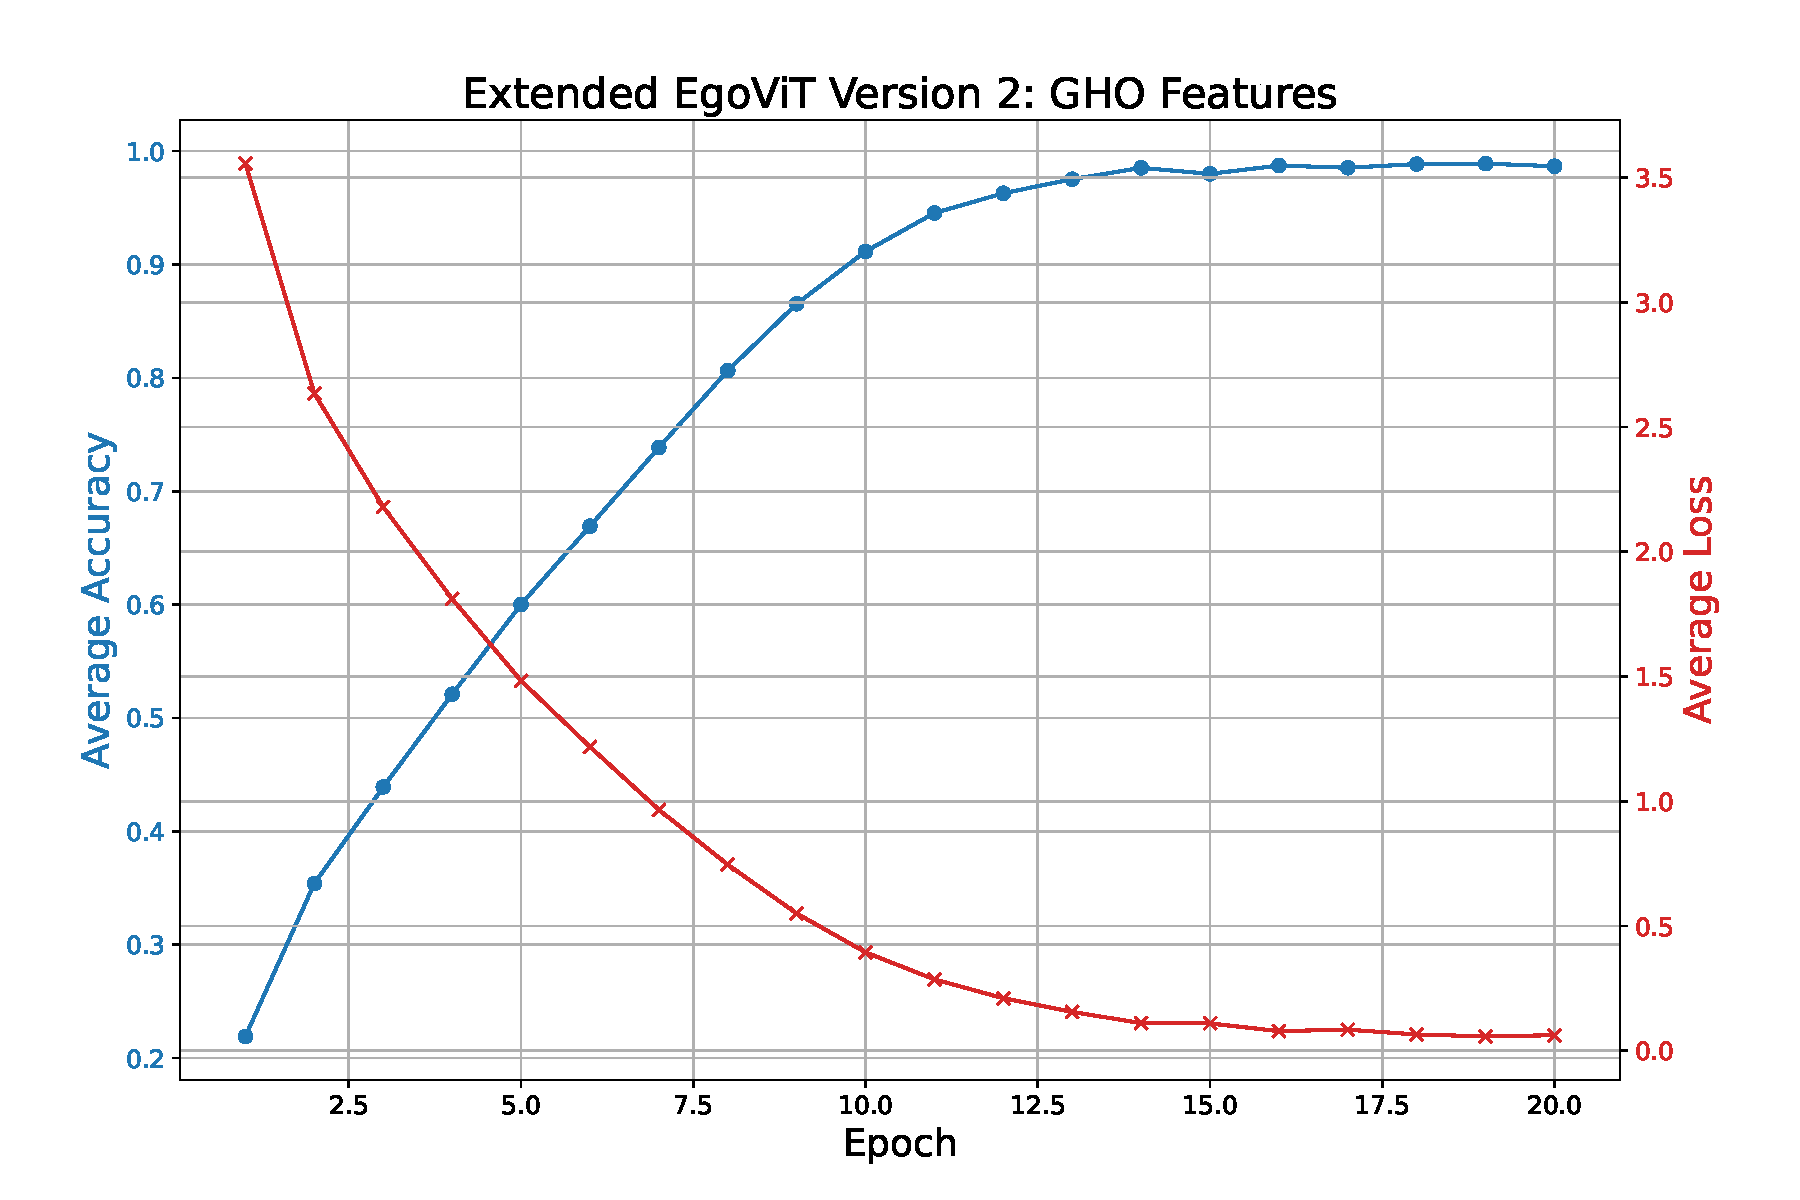
\includegraphics[width=0.9\textwidth]{graphics/figure6}
    \caption{Training loss and accuracy of the enhanced EgoViT version 2 with gaze-hand-object features. Blue curve: training accuracy, red curve: training loss.}
    \label{fig:egovit_v2_GHO}
\end{figure}
\vspace{3mm}
The training loss and accuracy of the enhanced EgoViT version 2 with gaze-hand-object features are shown in Figure \ref{fig:egovit_v2_GHO}. Comparing with Figure \ref{fig:egovit-with-gho} the loss and accuracy curves of the two experiments are similar. They both reach the minimum loss after 15 epochs and have the kinks points at epoch 2 and 15. This training result indicates that the gaze features and hand-object features can be used as class tokens in the model and processed independently. This modification does not significantly affect the model's training performance.

The testing results of the enhanced EgoViT version 2 with gaze-hand-object features are shown in Table \ref{tab:Results_table4}. The model achieves a top-1 accuracy of 50.2\%, a top-5 accuracy of 75.8\%, and a mean class accuracy of 38.3\%. These results are lower than those of the experiment Enh\_GHO\_v2. This indicates that the modified \gls{dctg} and \gls{padm} modules do not improve the model's performance. 
\vspace{5mm}
\begin{table}[htbp]
    % \mycaption{Comparison of Test Results on EgoViT with gaze information}{ddd}
    \centering
    \caption{Comparison of Test Results on EgoViT with Gaze Information}
    \begin{tabular}{lccc}
    \hline\hline
    Training Method & Top-1 Acc.(\%)& Top-5 Acc.(\%)& Mean Class Acc.(\%) \\
    \hline
    Enh\_GHO\_v2 & 52.0 & 76.3 & 38.7 \\
    Enh\_v2\_GHO\_v2 & 50.4 & 75.8 & 38.3 \\
    \hline\hline
    \end{tabular}
    \label{tab:Results_table4}
\end{table}
\clearpage
The second variant, enhanced EgoViT version 3, has a different input configuration for the head. Both the weighted class token and the normal token from the long-term stage are directly fed into the head without separation. To evaluate the effect of this input configuration, the variant enhanced EgoViT version 3 is trained with hand-object features, gaze features, and gaze-hand-object features. The training loss and accuracy of the enhanced EgoViT version 3 with hand-object features, gaze-hand-object features, and only gaze features are shown in Figure \ref{fig:egovit_v3_HO}, \ref{fig:egovit_v3_GHO}, and \ref{fig:egovit_v3_G} respectively. They exhibit similar loss convergence curves, reaching the minimum loss after 15 epochs. 

Additionally, the training loss of experiments Enh\_GHO,  Enh\_GHO\_v2, and \\ Enh\_GHO\_v3 are compared in Figure \ref{fig:loss_comparison}. The loss curves of Enh\_GHO and Enh\_GHO\_v2 represented by lines with cross markers and lines with circle markers, exhibit a similar curve trend. The line with square markers represents Enh\_GHO\_v3, which converges more slowly between epochs 4 and 15. This result indicates that the input configuration of the head and independently processing gaze features and hand-object features in the short-term and long-term stages do not significantly affect the model's training performance.

\begin{figure}[htbp]
    \centering
    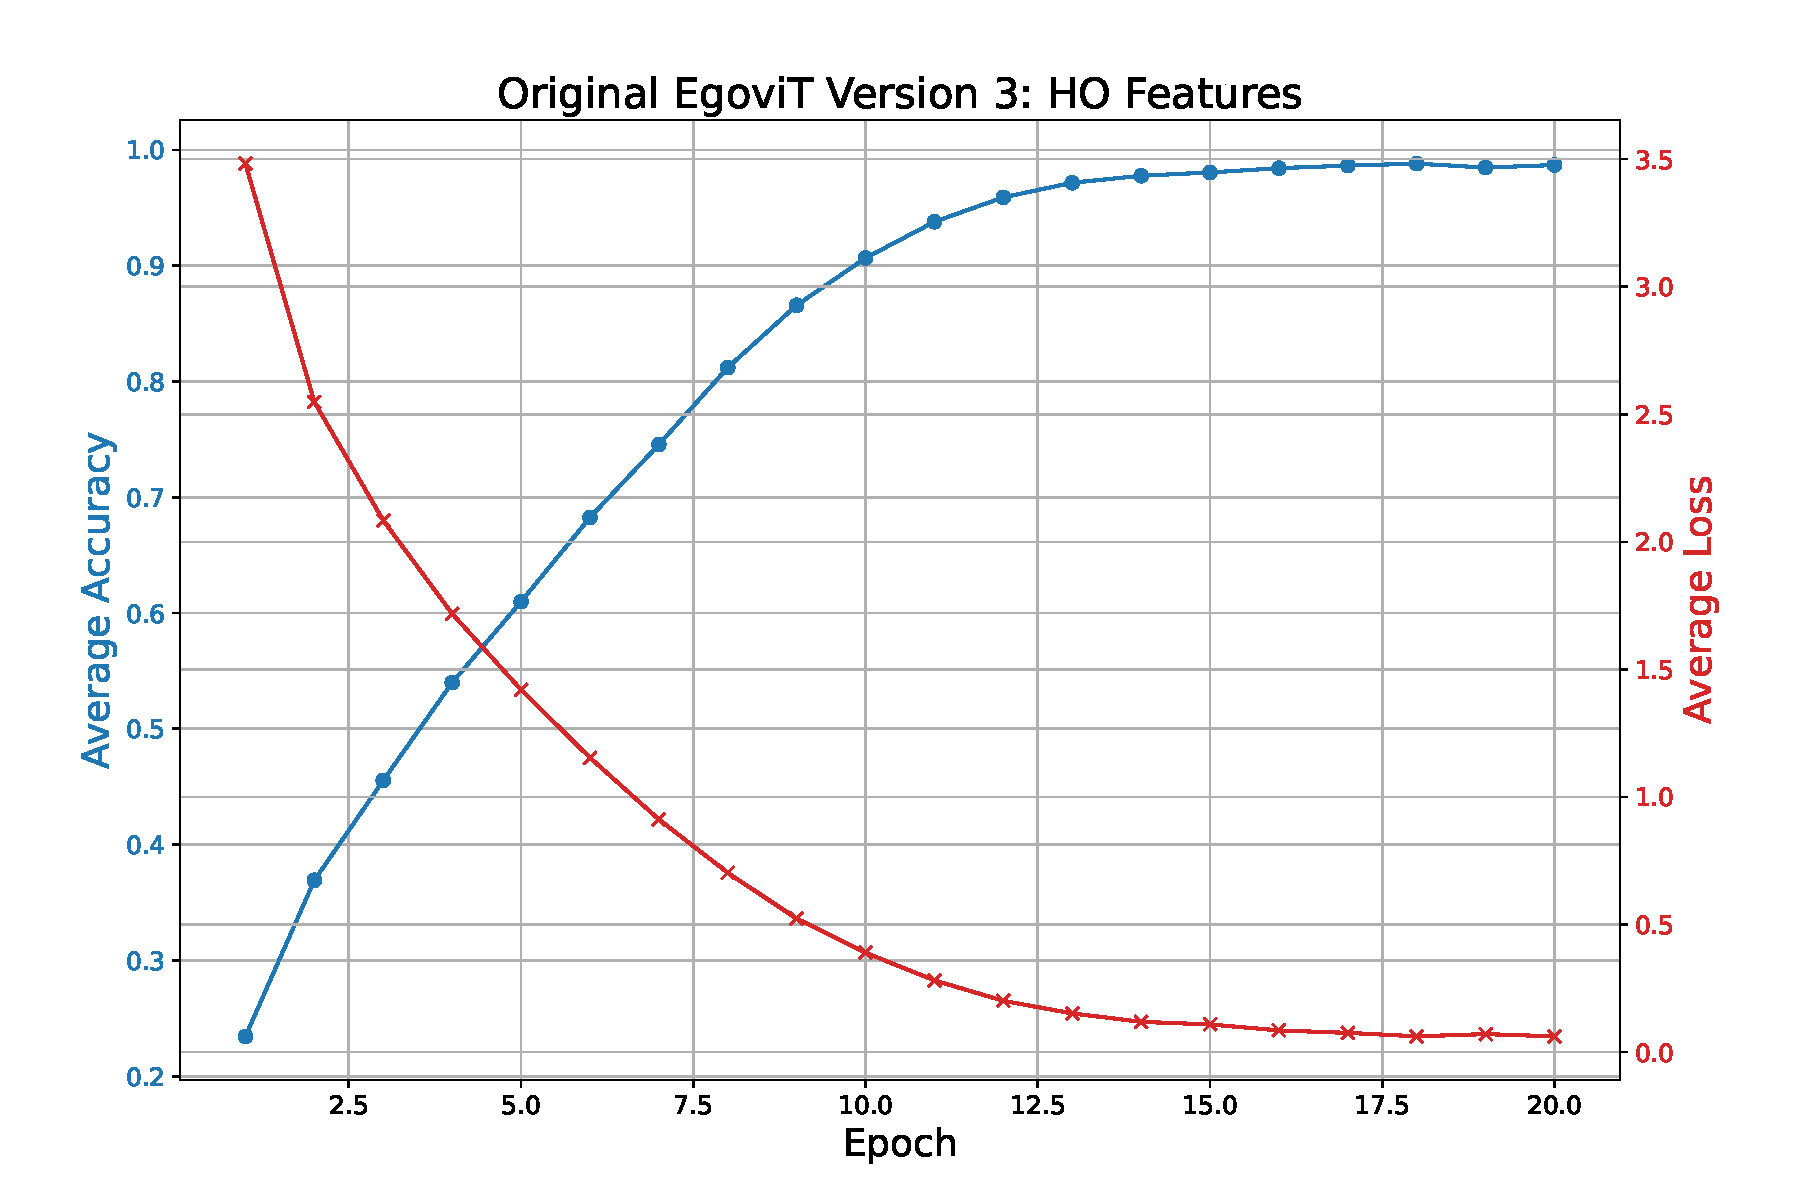
\includegraphics[width=0.9\textwidth]{graphics/figure7}
    \caption{Training loss and accuracy of the original EgoViT version 3 with hand-object features. Blue curve: training accuracy, red curve: training loss.}
    \label{fig:egovit_v3_HO}
\end{figure}
\clearpage
\begin{figure}
    \centering
    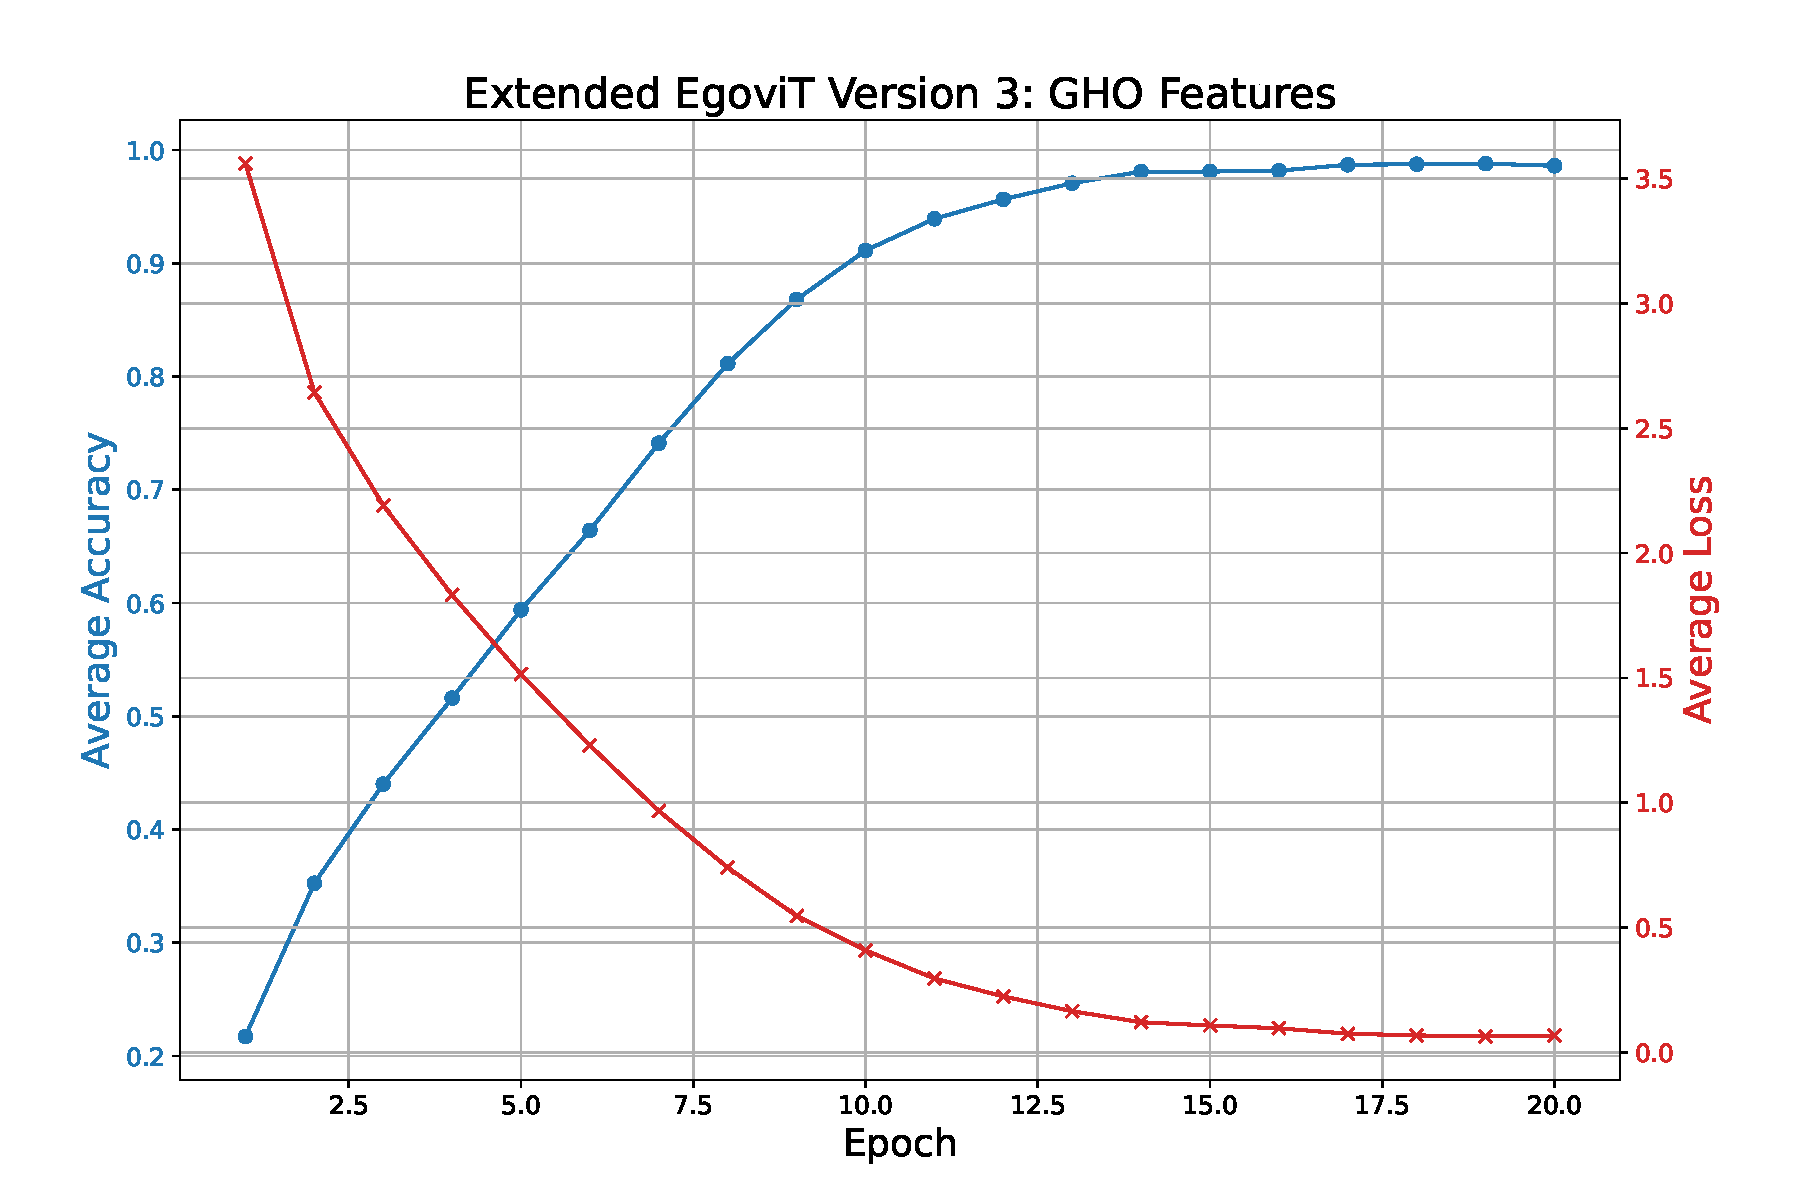
\includegraphics[width=0.9\textwidth]{graphics/figure8}
    \caption{Training loss and accuracy of the enhanced EgoViT version 3 with gaze-hand-object features. Blue curve: training accuracy, red curve: training loss.}
    \label{fig:egovit_v3_GHO}
\end{figure}
\begin{figure}
    \centering
    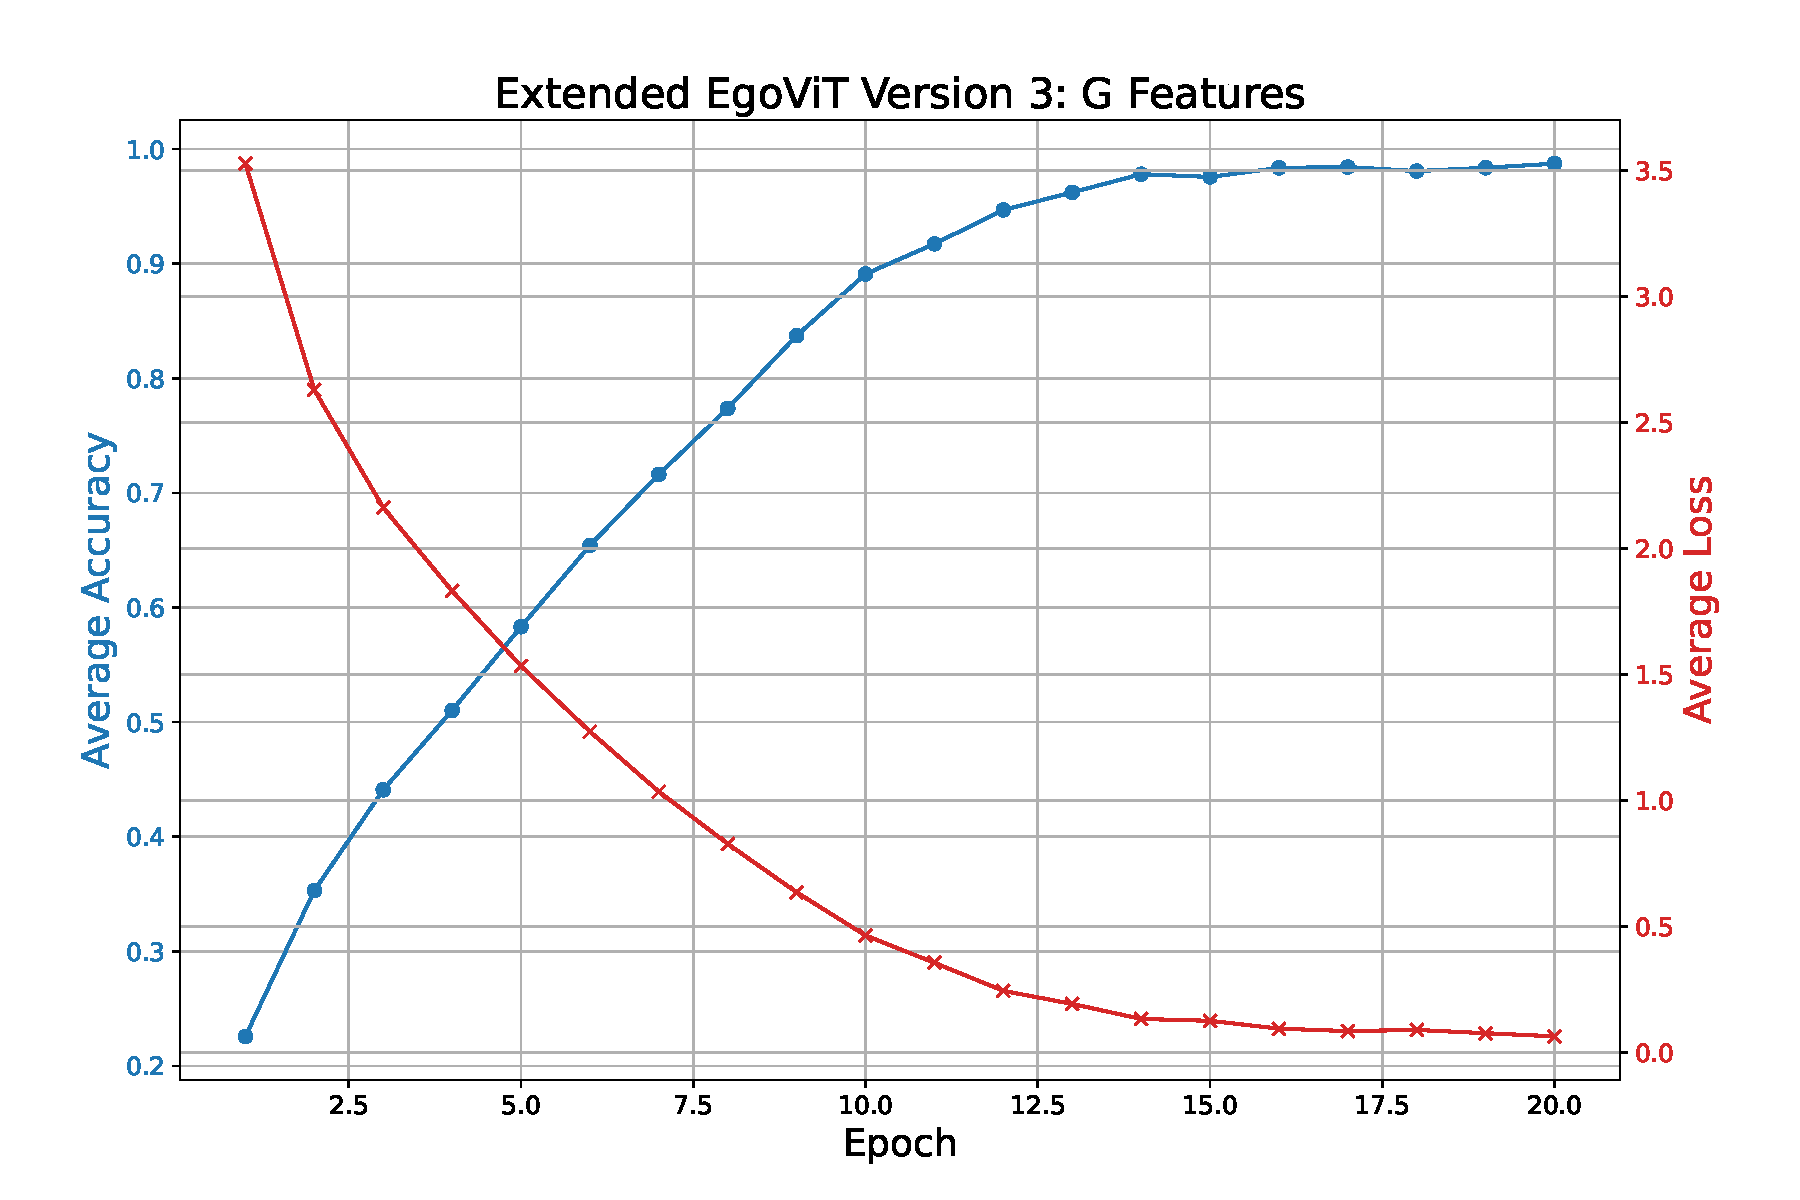
\includegraphics[width=0.9\textwidth]{graphics/figure9}
    \caption{Training loss and accuracy of the enhanced EgoViT version 3 with gaze features. Blue curve: training accuracy, red curve: training loss.}
    \label{fig:egovit_v3_G}
\end{figure}
\clearpage
\begin{figure}[htbp]
    \centering
    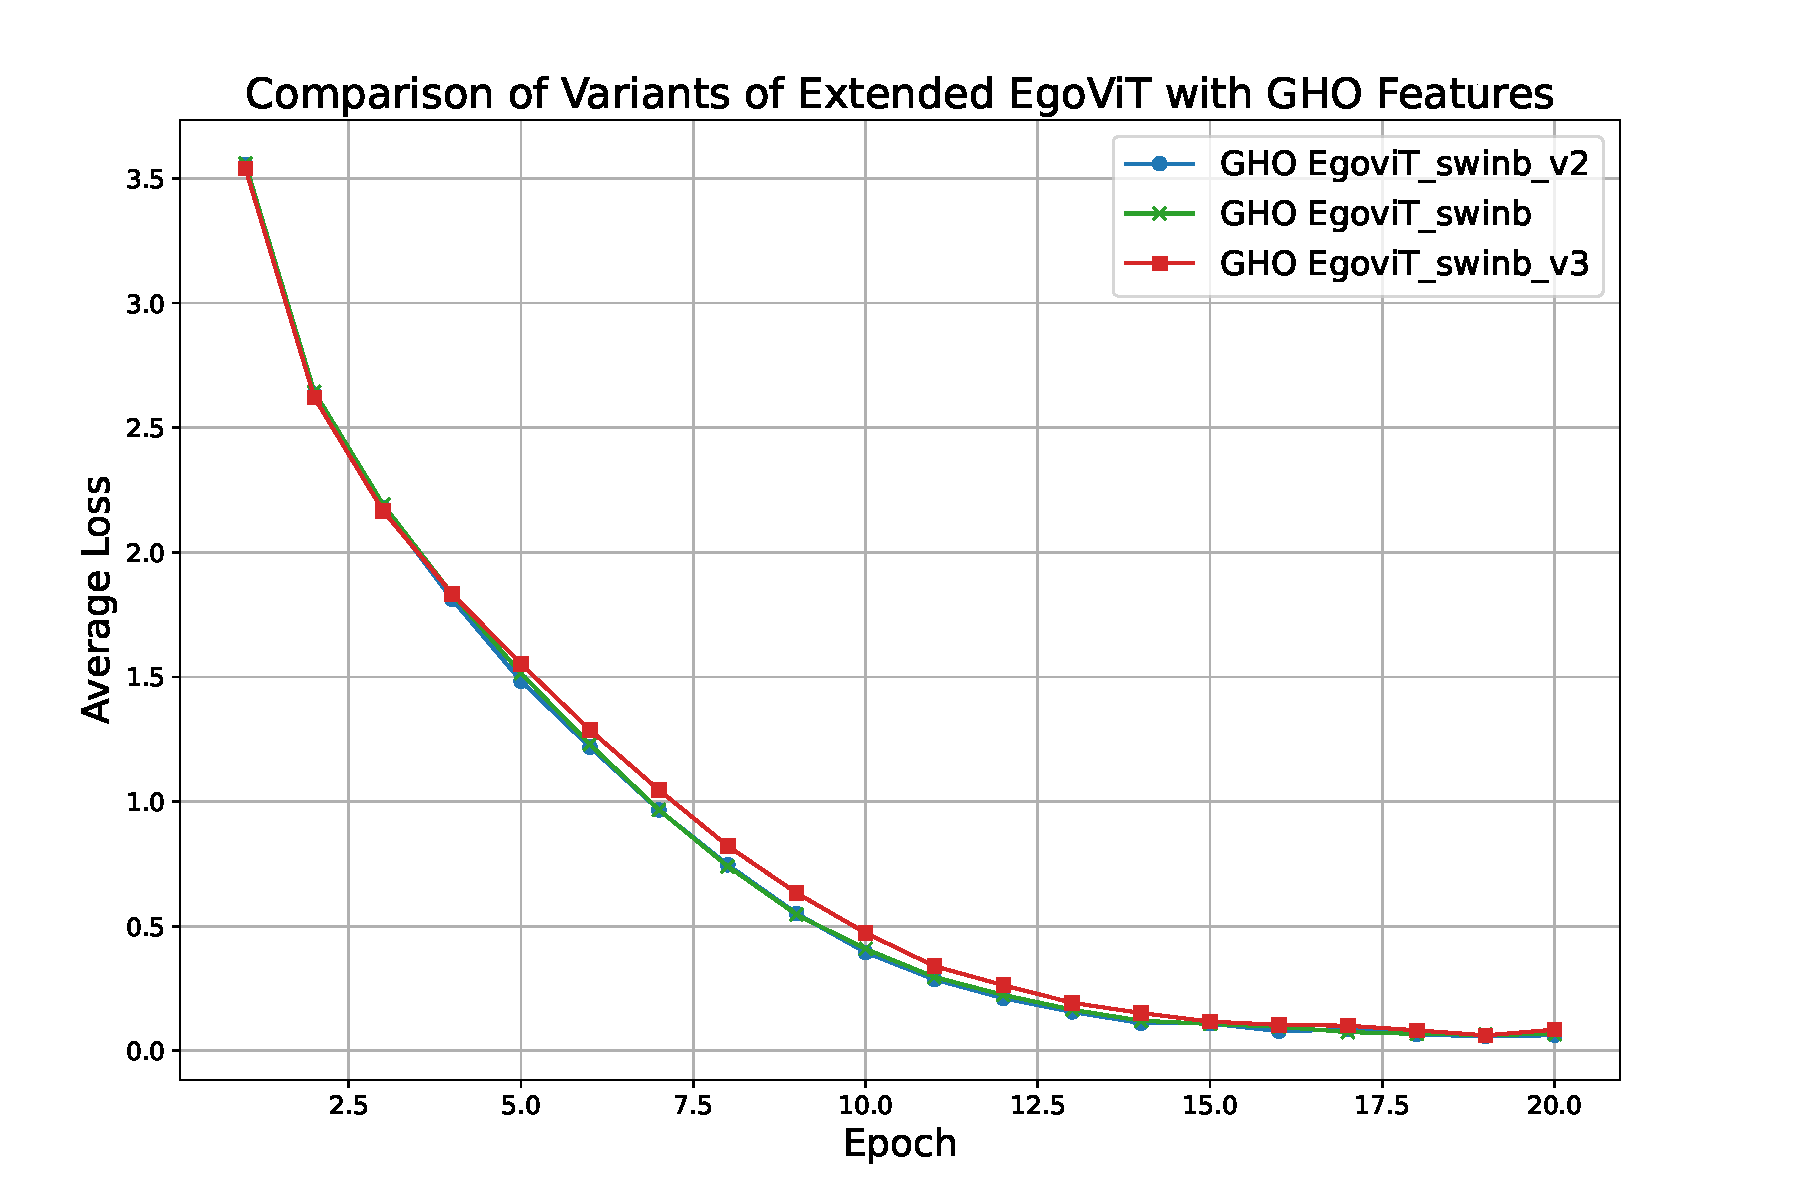
\includegraphics[width=0.9\textwidth]{graphics/loss}
    \caption{Comparison of training loss of the variants of enhanced EgoViT with gaze-hand-object features.}
    \label{fig:loss_comparison}
\end{figure}
% \vspace{5mm}
\begin{table}[htbp]
    \centering
    \caption{Test Results on EgoViT Version 3 Trained on Different Features}
    \begin{tabular}{lccc}
    \hline\hline
    Experiment ID & Top-1 Acc.(\%)& Top-5 Acc.(\%)& Mean Class Acc.(\%) \\
    \hline
    Orig\_v3\_HO & 51.1 & 77.4 & 40.5 \\
    Enh\_v3\_GHO\_v2 & 51.2 & 77.9 & 39.2 \\
    Enh\_v3\_G\_v2   & 50.8 & 75.9 & 37.8 \\
    \hline\hline
    \end{tabular}
    \label{tab:Results_table5}
\end{table}
\vspace{5mm}
The testing results of the enhanced EgoViT version 3 with hand-object features, gaze-hand-object features, and only gaze features are shown in Table \ref{tab:Results_table5}. The experiment orig\_v3\_GHO achieves the highest top-1 and top-5 accuracy of 51.2\% and 77.9\%, respectively. However, However, the results are almost the same as those of the experimen Orig\_v3\_HO, with only 0.1\% and 0.5\% higher top-1 and top-5 accuracy, respectively. The experiment Enh\_v3\_G\_v2 achieves the loswest accuracy across all three metrics. This result indicates that the input configuration of the head does not significantly affect the \gls{ear} performance.

\section{Disscussion}
\label{sec:Disscussion}
The results of all experiments are analyzed and discussed in this section. A comparison of the three metrics (top-1 accuracy, top-5 accuracy, and mean class accuracy) for all experiments is shown in Table \ref{tab:Results_all}, providing an overview of the inference results.

The experiments conducted in section \ref{sec:training_original_egovit} show that the original EgoViT performs better with pretrained weights from the Video Swin Transformer. Although the pretrained weights are trained on an image dataset and the architecture of the Video Swin Transformer is modified, the model with a fixed learning rate of $1 \mathrm{e}{-5}$ achieves better accuracy than the model with a scheduler learning rate as followed by \cite{liu_video_2021}. The configuration of the learning rate for different layers in the model has the potential to affect model accuracy, thus a new configuration could be explored in future work.

In experiments Enh\_GHO, Enh\_G, Enh\_GHO\_v2, and Enh\_G\_v2, two versions of gaze data are used for training. The results show that the model trained with gaze version 2 performs better than the model trained with gaze version 1. The quality of collected gaze tracking data significantly affects the model's performance, especially when only gaze information is used. The two additional experiments on the variants of the enhanced EgoViT show that the modified \gls{dctg} and \gls{padm} modules, as well as the input configuration of the head, do not improve the model's performance. One reason could be that the information in the class token, i.e., the gaze and hand-object features, are already exchanged with the normal token in the 3D Shifted \gls{msa} in the Video Swin Transformer. Therefore, even the gaze and hand-object features are processed independently in the short-term and long-term stages, the class token has the surfficient information for classification.

A noticeable obeservation is all experiments have a mean accuracy under 41\%, and the top-1 accuracy is only around 50\%. The sesults achieves lower performance than the Video Swin Transformer trained on other datasets. A plausible reason for this is that the EGTEA Gaze+ dataset is more challenging than other datasets. This dataset has an imbalanced distribution of samples in each class, with some classes having fewer than 40 samples. While class label 1 has about 600 samples. The model may not able to effectively learn the features of classes with fewer samples. 
\newpage
Although the dataset is challenging, the results of the experiment Enh\_GHO\_v2 shows a promising improvement in the performance of \gls{ear}. The enhanced EgoViT model trained with gaze-hand-object features achieves a top-1 accuracy of 52.0\% and a top-5 accuracy of 76.3\%. These results are higher than those of the original EgoViT model trained with hand-object features. This demonstrates that integrating additional gaze information can potentially improve \gls{ear} performance. The work in this thesis provides a foundation for future research on the use of gaze information in \gls{ear}.


\vspace{5mm}
\begin{table}[htbp]
    \centering
    \caption{Test Results of Various Experiments}
    \begin{tabular}{lccc}
    \hline\hline
    Experiment ID & Top-1 Acc.(\%)& Top-5 Acc.(\%)& Mean Class Acc.(\%) \\
    \hline
    Orig\_HO\_no\_pretrain & 51.5 & 78.5 & 38.8 \\
    Orig\_HO               & 51.7 & 75.2 & 40.6 \\
    Orig\_HO\_sched. LR    & 48.4 & 74.4 & 35.8 \\
    Enh\_ GHO           & 51.4 & 76.7 & 40.0 \\
    Enh\_G              & 48.9 & 75.1 & 37.7 \\
    Enh\_GHO\_v2        & 52.0 & 76.3 & 38.7 \\
    Enh\_G\_v2          & 50.0 & 76.2 & 38.0 \\
    Enh\_v2\_GHO\_v2    & 50.4 & 75.8 & 38.3 \\
    Enh\_v3\_HO         & 51.1 & 77.4 & 40.5 \\
    Enh\_v3\_GHO\_v2    & 51.2 & 77.9 & 39.2 \\
    Enh\_ v3\_G\_v2     & 50.8 & 75.9 & 37.8 \\
    \hline\hline
    \end{tabular}
    \label{tab:Results_all}
\end{table}